% =====================================================================
% DUAL-MAINTAINED FILE.
%
% This .tex and docs/drafts/task-model-paper.md are kept in parallel.
% The .md is shorter (skeleton + headline numbers); the .tex carries the
% full submission prose. Substantive prose changes that originate in the
% .tex must be mirrored back to the .md before commit (and vice versa).
%
% Pandoc regeneration is not currently in the pipeline because the .md
% is too skeletal to round-trip; treat the two files as parallel
% artifacts with synchronized intent.
%
% Edit history (recent):
%   - 2026-04-26 NB13 K1–K7 numbers and NB07a K1 (69%) updated in both files.
%   - 2026-04-26 §5.7 motor pillar recomputed against post-2026-04-12
%     fixation-y bugfix (44 px overall gap, 37/46 participants in predicted
%     direction). §5.8 position-9 fixation uptick retired in both files
%     (failed participant clustering).
%   - 2026-04-27 reframe to single-strand rational-analysis lineage
%     (Anderson → Pirolli & Card → SNIF-ACT → OSEC) with Zhang & Gwizdka
%     2016 / Z&AS 2018 as convergent decomposition from the economic-IR
%     tradition (Stigler/Varian/Azzopardi). Both abstract, §1, §2, §6.2,
%     §7 mirrored.
% =====================================================================

\documentclass[10pt,twocolumn,letterpaper]{article}

% --- Packages ---
\usepackage[utf8]{inputenc}
\usepackage[T1]{fontenc}
\usepackage{lmodern}
\usepackage[margin=0.65in,top=0.75in,bottom=0.65in]{geometry}
\usepackage{amsmath}
\usepackage{amssymb}
\usepackage{graphicx}
\usepackage{booktabs}
\usepackage{float}
\usepackage{hyperref}
\usepackage{xcolor}
\usepackage{caption}
\usepackage{natbib}
\usepackage{microtype}

% Compact spacing
\setlength{\parskip}{1.5pt plus 1pt}
\setlength{\parindent}{0.5em}
\setlength{\abovecaptionskip}{4pt}
\setlength{\belowcaptionskip}{2pt}
\setlength{\textfloatsep}{6pt}
\setlength{\floatsep}{4pt}
\setlength{\dbltextfloatsep}{6pt}

% Compact sections
\makeatletter
\renewcommand\section{\@startsection{section}{1}{\z@}{5pt}{2pt}{\normalfont\bfseries\normalsize}}
\renewcommand\subsection{\@startsection{subsection}{2}{\z@}{3pt}{1.5pt}{\normalfont\bfseries\small}}
\makeatother

% Compact abstract
\renewenvironment{abstract}{\small\noindent\textbf{Abstract.}\enspace\ignorespaces}{\par\vspace{4pt}}

\hypersetup{colorlinks=true, linkcolor=blue!70!black, citecolor=blue!70!black, urlcolor=blue!70!black}

\title{\vspace{-8pt}\textbf{Orient--Survey--Evaluate--Commit:\\A Cognitive Task Model for SERP Evaluation}\\[4pt]
{\normalfont\small\textcolor{gray}{Preprint --- under revision}}\vspace{-4pt}}

\author{
  Andy Edmonds\\[-2pt]
  {\small Independent Researcher, San Francisco, CA}\\[-2pt]
  {\small\texttt{andyed@alum.cmu.edu}}
}

\date{\vspace{-4pt}\small Draft of \today\vspace{-8pt}}

\begin{document}
\maketitle

% ============================================================
\begin{abstract}
We propose a four-phase cognitive task model for SERP evaluation---\textsc{Orient}, \textsc{Survey}, \textsc{Evaluate}, \textsc{Commit}---in the rational-analysis tradition that runs from Anderson~\cite{anderson1990adaptive,anderson1991reflections} through Pirolli \& Card's information foraging~\cite{pirolli1999foraging} and Fu \& Pirolli's SNIF-ACT~\cite{fu2007snifact}. The model takes that lineage to saccade-level granularity, grounded in eye-tracking evidence from 2,776 product search trials (AdSERP dataset, 47 participants). Saccade amplitude analysis identifies the \textsc{Survey} phase as ${\sim}3.5$ wide saccades ($107.8$\,px median) over ${\sim}1$\,s, during which users sample the result set before committing to reading. The survey--evaluate transition is marked by an amplitude drop detectable at $p = 9.3 \times 10^{-168}$ within individual trials ($N = 2{,}754$). Survey duration is fixed and does not respond to SERP content, but its output---an impression of result set composition---modulates subsequent evaluation strategy. The Survey/Evaluate split converges with a structurally analogous decomposition arrived at independently from the economic-IR tradition: Zhang \& Gwizdka's PCA on search-cost variables~\cite{zhang2016rethinking} recovers exploratory and validation processes that map onto Survey and Evaluate, and Zhang, Abualsaud \& Smucker~\cite{zhang2018requery} hypothesize a result-inspection phase consistent with the same mechanism. We operationalize SERP difficulty as \emph{relevance spread} (variance in query-result embedding similarity) and show it predicts page coverage, click position, and trial duration within-participant. The model adds a within-evaluation axis neither tradition has decomposed: \emph{forward} evaluation and \emph{regressive} re-evaluation are distinct sub-processes within the same task, with cursor-gaze coupling tighter for regressive than forward fixations across acquisition, evaluation, and scanning windows ($37/46$ participants in the predicted direction; Wilcoxon $p = 4.8 \times 10^{-5}$).
\end{abstract}

% ============================================================
\section{Introduction}

Information search has been analyzed as a cost-rational adaptation since Anderson's rational analysis of cognition~\cite{anderson1990adaptive}, which frames cognitive performance as cost-optimized to the structure of the environment. Anderson \& Schooler~\cite{anderson1991reflections} model memory retrieval probability as a Bayesian function of environmental need probability---retrieval as relevance estimation. Pirolli \& Card's information foraging theory~\cite{pirolli1999foraging} operationalizes this account for information search: scent-driven patch assessment with marginal-value-theorem stopping. Fu \& Pirolli's SNIF-ACT~\cite{fu2007snifact} gives the framework an ACT-R implementation in which the patch-leaving decision is spreading activation over scent values. The granularity beneath SNIF-ACT---saccade-level decomposition of within-SERP evaluation cost---has not yet been reached.

Click models~\cite{craswell2008positionbias,chapelle2009dbn,dupret2008ubm,chuklin2015clickmodels} parameterize examination and stopping but do not connect their parameters to the rational-analysis lineage. Cursor-feature classifiers extract feature bags from mouse trajectories~\cite{arapakis2016engagement}; transformer sequence models learn end-to-end maps from raw $(x, y, t)$ to click~\cite{villaizan2025adsight,bruckner2021systematic}. These deliver real engineering gains but treat user behavior as a signal to decode rather than as a cost-allocation process. We model that process explicitly with a four-phase cognitive task model for SERP evaluation---\textsc{Orient}, \textsc{Survey}, \textsc{Evaluate}, \textsc{Commit}---with measurable transitions between phases and a within-evaluation \emph{forward}/\emph{regressive} axis no prior account has decomposed.

Each phase in the model has precedent in the literature taken in isolation. Orientation is implicit in click models' position-bias assumptions. Scanning-then-reading appears in Liu et al.'s two-stage examination model~\cite{liu2014skimming}. The \textsc{Survey} phase converges with two findings from a different theoretical backbone---the economic-IR cost-modeling tradition (Stigler 1961, Varian 1999, Azzopardi~\cite{azzopardi2011economics,azzopardi2014modelling}): Zhang \& Gwizdka's~\cite{zhang2016rethinking} factor-analytic decomposition of search cost into exploratory and validation processes, and Zhang, Abualsaud \& Smucker's~\cite{zhang2018requery} mechanistic hypothesis of a result-inspection phase. Committed evaluation is the subject of decades of relevance-assessment research. Satisficing as a stopping rule is central to the foraging account. Scroll regressions are documented by Lorigo et al.~\cite{lorigo2008eyetracking}. The contribution is the synthesis: identifying these as phases of a single task with measurable transitions, and adding a within-evaluation forward/regressive axis that no prior account in either tradition has decomposed.

The empirical anchor is a saccade amplitude transition at fixation ${\sim}5$ ($p = 9.3 \times 10^{-168}$, $N = 2{,}754$ trials), operationalizing the survey phase Zhang et al.\ hypothesized seven years earlier. Click models cannot see this because they examine clicks, not saccades; end-to-end cursor learners cannot see it because they lack the task-level concept of a phase boundary to look for. The decomposition is recoverable only if the analyst is looking for phase structure in the first place.

We test the decomposition on a forced-choice product search task (AdSERP) that eliminates two of the three natural exit paths from SERP evaluation---reformulation and abandonment. This isolates the orient--survey--evaluate--commit sequence but cannot characterize the full foraging decision (stay, refine, or quit). Validating the complete model requires production log data with natural stopping behavior.

% ============================================================
\section{Related Work}

OSEC sits inside a three-decade lineage that has progressively decomposed search cost at finer and finer granularities. We review the lineage explicitly, then turn to what has \emph{not} yet been decomposed---the within-evaluation forward/regressive axis that this paper adds.

\subsection{Rational-analysis cognitive psychology of search}
\label{sec:lineage}
The model sits in the rational-analysis tradition that runs from Anderson through Pirolli \& Card. Anderson~\cite{anderson1990adaptive} frames cognitive performance as cost-optimized adaptation to the structure of the environment. Anderson \& Schooler~\cite{anderson1991reflections} provide the empirical instantiation: memory retrieval probability tracks the environmental statistics of need probability---retrieval as relevance estimation. Pirolli \& Card's information foraging theory~\cite{pirolli1999foraging} operationalizes the account for information search: scent-driven patch-quality assessment with marginal-value-theorem stopping. Fu \& Pirolli's SNIF-ACT~\cite{fu2007snifact} gives the framework an ACT-R implementation in which patch-leaving is spreading activation over scent values. Brumby \& Howes~\cite{brumby2004goodenough} capture a fast/slow two-phase structure (``good enough but I'll just check'') consistent with the same lineage. Satisficing with aspiration levels (Payne \& Duggan, following Simon) models the commit decision as a threshold crossing rather than an optimization. Each rung operationalizes search behavior at a finer granularity. OSEC takes the granularity below SNIF-ACT: saccade-level decomposition of within-SERP evaluation cost, with phase boundaries identifiable trial-by-trial.

\subsection{Convergent decomposition from the economic-IR tradition}
\label{sec:convergent}
A separate research tradition arrives at a structurally analogous decomposition by a different route. Stigler's economics of information~\cite{stigler1961economics} and Varian's SIGIR 1999 keynote~\cite{varian1999economics} opened a cost-economic line in IR that Azzopardi's economic models of interactive retrieval~\cite{azzopardi2011economics,azzopardi2014modelling} formalized: production costs (per-query, per-snippet, per-document inspection), benefit functions (relevance returned per unit time), and stopping rules derived from microeconomic theory. Zhang \& Gwizdka~\cite{zhang2016rethinking} took this line empirical: a PCA of six search-cost variables (time and word-count on unproductive queries, SERP fixation count, time and fixation-count on the task description, fixation-count on unproductive documents) recovered two well-separated factors with cross-loadings near zero, which they labelled \emph{exploratory process} (loading on query-issuing and SERP scanning) and \emph{validation process} (loading on task-description re-reading and unproductive-document reading), and mapped onto Kuhlthau's Initiation/Selection/Exploration vs Formulation/Collection stages and Marchionini's Define/Select/Formulate/Execute vs Examine Results stages.

The decomposition is structurally analogous to a Survey-then-Evaluate split, recovered at participant-aggregate granularity from search-cost variables alone. The two traditions share no central citations: Anderson, Pirolli \& Card, and SNIF-ACT do not appear in Zhang \& Gwizdka's reference list, and Stigler, Varian, and Azzopardi are absent from the rational-analysis literature OSEC inherits from. That two independently developed cost frameworks---one psychological, one economic---recover the same two-factor decomposition is a robustness signal for the decomposition itself: not a single tradition's idiosyncratic carving of the data, but a structure that survives translation across vocabularies. Zhang, Abualsaud \& Smucker's~\cite{zhang2018requery} mechanistic hypothesis of a ``result inspection phase'' gating the stay-or-reformulate decision is consistent with the same survey-phase structure at the per-trial decision level.

We note one cost-variable mismatch with the economic-IR factor structure: Zhang \& Gwizdka's \emph{exploratory} factor includes the cost of generating new queries, which OSEC does not (query generation is upstream of \textsc{Orient}); their \emph{validation} factor includes task-description re-reading, which has no OSEC analog. The mappings are analogous, not identical---the convergence is on structure, not on cost-variable composition.

\subsection{Process models of information seeking}
The HCI and information-science tradition models search as a process with identifiable stages. Kuhlthau's Information Search Process (ISP) identifies six affective and cognitive stages across a multi-session inquiry. Marchionini's eight sub-processes decompose a single search episode into recognize, accept, define, select, formulate, execute, examine, extract. Bates's berrypicking abandons the single-query assumption and models search as an evolving sequence of refinements. Belkin's Anomalous State of Knowledge frames the whole activity as a cognitive gap-closing operation. These models are powerful at the session scale and anchor the HCI/IS view of search behavior, but they are too coarse to predict what happens during the 3--30 seconds between SERP render and first click. Zhang \& Gwizdka's~\cite{zhang2016rethinking} factor-analytic decomposition (\S\ref{sec:convergent}) brought them down one level. Our work continues that descent.

\subsection{Click models as implicit cost models}
The IR click-modeling tradition encodes assumptions about cost without labelling them as such. The cascade model~\cite{craswell2008positionbias} assumes serial top-down examination with a stopping rule---in cost-decomposition vocabulary, an undifferentiated cost-allocation policy that pays per-position inspection cost and stops when the running benefit clears a threshold. The Dynamic Bayesian Network click model~\cite{chapelle2009dbn} adds per-position skip/examine decisions that implicitly modulate the inspection-cost rate. The User Browsing Model~\cite{dupret2008ubm} parameterizes position-dependent examination probability and, through the distance-to-last-click term, implicitly models orientation cost. The comprehensive survey by Chuklin et al.~\cite{chuklin2015clickmodels} makes the pattern visible across the family. Every one of these models is a parameterized cost-allocation policy without explicit cognitive grounding. Connecting their parameters to the cost-rational lineage of \S\ref{sec:lineage}---instead of fitting them in isolation---is the route to interpretable parameters that compose, validate against behavioral data, and transfer across paradigms.

\subsection{Two-stage examination models}
Liu et al.~\cite{liu2014skimming} provide the closest finer-granularity empirical precedent for the Survey/Evaluate split: a two-stage examination model in which users skim a SERP before reading specific results, with both stages predictable from cursor data. Our model adds \textsc{Orient} before skimming and decomposes Liu et al.'s ``skimming'' into \textsc{Survey} (gist sampling, wide saccades) and early \textsc{Evaluate} (committed reading, narrow saccades), with a saccade-amplitude marker for the phase boundary. Brumby \& Howes~\cite{brumby2004goodenough} (\S\ref{sec:lineage}) capture the same fast/slow structure within the rational-analysis lineage at a different task. Zhang, Abualsaud \& Smucker's~\cite{zhang2018requery} result-inspection-phase hypothesis (\S\ref{sec:convergent}) is the same survey-phase mechanism observed in the requery context. Our contribution relative to these precedents is saccade-level measurement that pulls the phase into a continuous trial-by-trial structure.

\subsection{Eye tracking on SERPs}
The eye-tracking literature has been describing phase structure since the mid-2000s without naming it. Granka et al.~\cite{granka2004eyetracking} reported an initial rapid scan followed by re-examination---phase structure in the data, unformalized. Cutrell \& Guan~\cite{cutrell2007eyetracking} showed that snippet length shifts evaluation effort, which we read as the survey phase setting the cost budget for the evaluate phase. Lorigo et al.~\cite{lorigo2008eyetracking} reported that ${\sim}2/3$ of SERP scanpaths are non-sequential, challenging the cascade assumption and consistent with a survey phase sampling several positions before committed reading. Buscher, Dumais \& Cutrell~\cite{buscher2010goodbad} documented distinct ad vs.\ organic fixation patterns, which our companion work~\cite{arapakis2016engagement} extends to a discrimination-cost argument at the cursor level. The phase structure is in the data; what has been missing is a task-model vocabulary that lifts it into a form click models can consume.

\subsection{The forward/regressive axis at SERP-evaluation granularity}
\label{sec:fwd-reg-gap}
Within-SERP forward and regressive evaluation has not been decomposed at task-model granularity by either tradition this paper draws on. The rational-analysis lineage (\S\ref{sec:lineage}) is mode-agnostic at the within-patch level: Pirolli \& Card model patch-leaving as a directional decision but do not split within-patch fixations by direction; SNIF-ACT's spreading-activation account is direction-neutral. The economic-IR lineage (\S\ref{sec:convergent}) parameterizes unit costs without distinguishing forward inspection from regressive re-inspection, and Zhang \& Gwizdka's PCA pools all SERP fixations into a single $F_{SERP}$ variable. Liu et al.'s two-stage examination distinguishes skimming from reading temporally, not directionally.

Two adjacent literatures formalize forward/regressive at different granularities. Reading research---reviewed by Rayner~\cite{rayner1998eyemovements}---models word-sequence regressions explicitly: roughly 10--15\% of fixations during text reading are saccadic regressions used to recover comprehension, and process models like E-Z Reader formalize their dynamics. Our forward/regressive split is at SERP-evaluation granularity using a scroll-position high-water-mark classifier, not within-result-saccade direction; the constructs are related but not identical. In the IR-evaluation tradition, the C/W/L framework~\cite{moffat2017cwl} models per-rank continuation probability as the stay/leave decision, decomposing examination effort by rank but not by direction within rank. The within-SERP forward/regressive split sits in the space between: it is the within-patch direction axis that reading research formalizes for word sequences and that IR-evaluation models leave folded into rank-level continuation. We treat forward and regressive evaluation as task-level modes with separate motor, pupillometric, and geometric signatures (\S\ref{sec:fwd-reg}), not as a saccade-classification artifact.

\subsection{Task analysis in HCI}
The methodology for decomposing tasks into cognitive, perceptual, and motor operators has existed since GOMS (Card, Moran \& Newell, 1983). Hornof \& Kieras's CPM-GOMS analyses of menu search show interleaved systematic and opportunistic scanning within a single display---directly analogous to our survey plus evaluate decomposition, applied decades ago at a slightly different granularity. Gray et al.'s soft-constraints hypothesis~\cite{gray2006soft} provides the rational-analysis framing at the millisecond scale, treating microstrategy selection as cost-optimized resource allocation. The methodology and vocabulary both exist; bringing them to bear on SERP evaluation at the 3--30 second granularity, in a form click models can consume, is the connecting move this paper attempts.

% ============================================================
\section{The Model}
\label{sec:model}

\begin{figure*}[t]
  \centering
  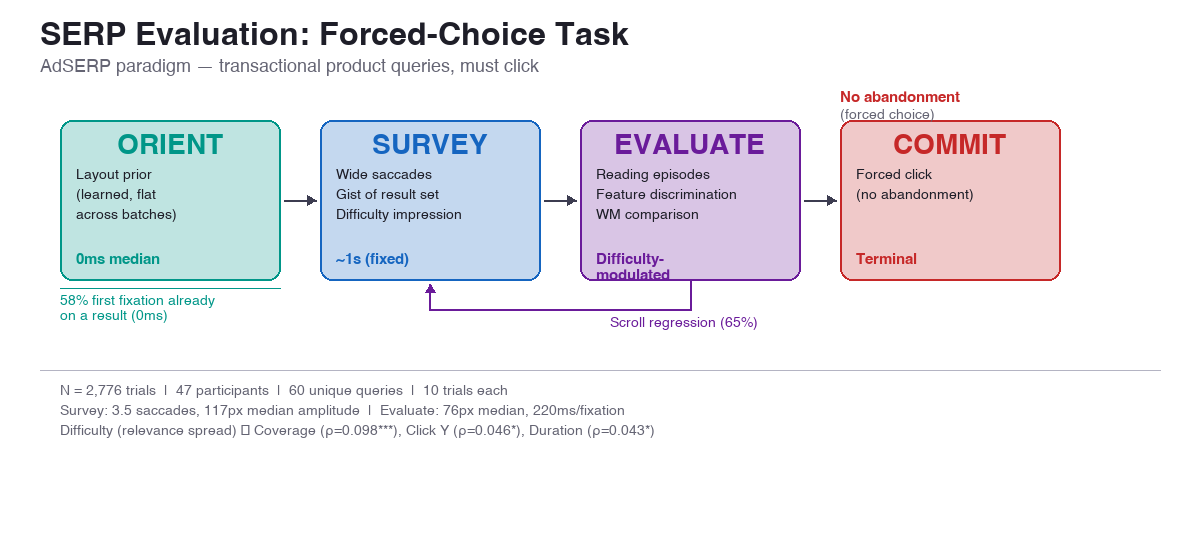
\includegraphics[width=\textwidth]{figures/task-model-adserp.png}
  \caption{Orient--Survey--Evaluate--Commit task model as instantiated for the AdSERP forced-choice paradigm. Orient is collapsed (learned prior, 0\,ms median). Survey is fixed-duration (${\sim}1$\,s). Evaluation duration is modulated by the difficulty impression formed during survey. No abandonment path (forced click).}
  \label{fig:model}
\end{figure*}

\subsection{Orient}
Layout recognition. For familiar SERP layouts, this is a learned prior: 58\% of AdSERP trials show first fixation already on a result (0\,ms orientation). No learning effect across 60 trials ($\rho = 0.02$, $p = 0.30$).

\subsection{Survey}
Wide saccades (107.8\,px median), ${\sim}3.5$ fixations, ${\sim}1$\,s. Gist sampling: the user builds an impression of result set composition without committed reading. Duration is \emph{fixed}---does not correlate with any difficulty measure (all $p > 0.3$). The survey's output, not its duration, modulates subsequent behavior.

\subsection{Evaluate}
Narrow saccades (69.4\,px median). Consecutive fixations on the same result connected by minor saccades ($<100$\,px) form \emph{reading episodes}: mean 2.16 fixations, 499\,ms. Per-fixation duration is flat (${\sim}220$\,ms across all positions). The position effect in total fixation time is driven by fixation count, not processing speed. Forward-only dwell \emph{increases} with position ($\rho = +0.82$), consistent with growing comparison-set size under framework compilation (per-position cognitive load \emph{decreases}; see Butterworth LF/HF validation).

\subsection{Commit}
Click. Satisficing threshold crossed. In AdSERP (forced choice), every trial ends with a click. In naturalistic search, this phase competes with abandonment and query reformulation.

\subsection{Regression loop}
69\% of trials include at least one scroll regression (1{,}566 / 2{,}266 trials; Evaluate $\rightarrow$ re-Survey). Backward scrolling is ballistic ($\rho = 0.867$), with 87\% of regression targets at positions 0--4.
% H3 dropped 2026-04-13: removed the "regression velocity mediates the dwell delta (rho = -0.762, p = 0.017)" claim.
% Reasons: (1) tiny N = 9 positions — same survivor-bias trap covered in methodological-threats.md §8;
% (2) "mediation" overclaims — the test is a Spearman correlation, not a Baron-Kenny mediation analysis;
% (3) p = 0.017 is borderline and does not survive Bonferroni across the multiple kinematics tests in
% the source notebook (notebooks/scroll_kinematics.ipynb). The ballistic-backscroll claim above carries
% the load on its own.

% ============================================================
\section{Data and Methods}

\subsection{AdSERP dataset}
AdSERP~\cite{latifzadeh2025adserp}: 2,776 trials, 47 participants, 60 unique product purchase queries (``buy [brand] [product]''). 10 trials per participant across 6 batches. Gazepoint GP3 HD eye tracker (150\,Hz). Fixations pre-segmented by the tracker's internal I-DT filter (FPOG stream). Mean single-fixation duration 218\,ms, median 187\,ms (N = 234{,}339 fixations across all trials, post 2026-04-12 coordinate-space audit; see NB04:K24--K27 for the canonical source).

\subsection{Saccade classification}
Saccade amplitude computed as Euclidean distance between consecutive fixation coordinates (FPOGX, FPOGY in screen pixels). Minor saccade threshold: 100\,px. Fixations $<60$\,ms filtered as sub-threshold artifacts (1.4\% of data).

\subsection{Phase identification}
Survey--evaluate transition: sliding window of 3 saccades. First window where mean amplitude $< 100$\,px marks the transition. Median transition at saccade 2 (51\% of trials transition within first 2 saccades).

\subsection{SERP difficulty measures}
Three measures computed per SERP:
\begin{itemize}\setlength\itemsep{0pt}
  \item \textbf{Jaccard:} mean pairwise token-set overlap across results (mean = 0.151)
  \item \textbf{Relevance spread:} std of query--result cosine similarity (mxbai-embed-large, 1024-d). Low spread = all results equidistant from query = hard (mean = 0.052). The precedent for treating variance across a retrieved set as a difficulty signal is the query performance prediction literature: Cronen-Townsend et al.'s clarity score~\cite{cronentownsend2002clarity} used divergence between query and collection language models, and Shtok et al.'s Normalized Query Commitment~\cite{shtok2012nqc} used the standard deviation of top-$k$ lexical retrieval scores. Both established that the shape of the retrieved-score distribution carries query-difficulty information. Relevance spread is the same primitive ported to dense embeddings and used here as a stimulus descriptor to test whether a system-side variance signal also predicts user-side behavioral variants (coverage, duration, click Y).
  \item \textbf{Distinctive density:} mean TF-IDF-weighted unique-token fraction per result (mean = 0.460)
\end{itemize}

Jaccard and relevance spread are strongly anti-correlated ($\rho = -0.450$), confirming they measure different constructs.

% ============================================================
\section{Results}

\subsection{Saccade amplitude distinguishes survey from evaluation}
Early saccades (fixations 1--5): 107.8\,px median (N = 13{,}840). Late saccades (fixations 6+): 69.4\,px median (N = 65{,}764). Survey/evaluate amplitude ratio 1.55$\times$. Per-trial amplitude slope over first 20 saccades: mean $\rho = -0.135$, $t = -29.63$, $p = 9.33 \times 10^{-168}$ ($df = 2{,}753$, $N = 2{,}754$ trials with $\geq 10$ saccades). 71.8\% of trials have $\rho < 0$.

\subsection{Orientation is a learned prior}
Median orientation time: 0\,ms (58\% of first fixations land on a result). No learning across batches ($\rho = 0.02$, $p = 0.30$). No within-participant trend ($\rho = -0.022$, $p = 0.26$).

\subsection{Survey duration is content-independent}
Mean 3.5 saccades, ${\sim}1$\,s. No correlation with relevance spread ($\rho = -0.000$), distinctive density ($\rho = 0.020$), or Jaccard ($\rho = -0.012$). All $p > 0.3$.

\subsection{Relevance spread predicts evaluation strategy}

\begin{table}[h]
\centering
\small
\caption{Spearman correlations: difficulty measure $\times$ behavioral DV ($N = 2{,}334$). Spread and density: positive $\rho$ = easier SERPs $\rightarrow$ more of DV.}
\label{tab:correlations}
\begin{tabular}{@{}lrrrrr@{}}
\toprule
& Dur. & Fix. & Cov. & Reg. & Click Y \\
\midrule
Jaccard  & $-.019$ & $-.021$ & $-.046^*$ & $.005$ & $-.055^{**}$ \\
Spread   & $.043^*$ & $.047^*$ & $\mathbf{.098^{***}}$ & $.035$ & $.046^*$ \\
Density  & $.014$ & $.015$ & $\mathbf{.071^{***}}$ & $.004$ & $-.052^*$ \\
\bottomrule
\end{tabular}
\end{table}

Within-participant: relevance spread $\rightarrow$ coverage ($\bar{\rho} = 0.089$, $p < 0.001$) and duration ($\bar{\rho} = 0.042$, $p = 0.031$).

Tercile analysis (relevance spread): hard SERPs (low spread) produce 49.0\% page coverage vs.\ 53.3\% for easy SERPs ($p < 0.001$). Click Y: 814\,px (hard) vs.\ 870\,px (easy, $p = 0.047$).

\subsection{Reading episodes and SERP difficulty}
Episode pooling (minor saccade threshold 100\,px): 95,328 episodes across 2,334 trials. 50.5\% single-fixation, 49.5\% multi-fixation (mean 2.16 fixations, 499\,ms). Proportion of multi-fixation episodes is higher on hard SERPs ($p = 0.004$).

\subsection{Fixation decomposition}
Per-fixation duration is flat at ${\sim}220$\,ms across positions 0--9 (range 202--228\,ms). Fixation count declines monotonically with organic rank (mean per-(trial, rank) fixation count $17.5 \rightarrow 13.4 \rightarrow 11.0 \rightarrow 9.3 \rightarrow 7.9 \rightarrow 6.9 \rightarrow 6.3 \rightarrow 5.4 \rightarrow 3.9 \rightarrow 3.4$ across organic ranks $0$--$9$; Spearman $\rho = -1.000$, $p = 5.5 \times 10^{-7}$, $N = 10$ ranks). Total dwell follows the same monotonic decline ($3.80 \rightarrow 0.80$\,s across the same ranks; $\rho = -1.000$, $p = 5.5 \times 10^{-7}$). The position effect in total fixation time is therefore carried by fixation count, not per-fixation duration---consistent with allocation rather than a processing-speed change. (Both correlations are computed on the full corpus of $2{,}776$ trials; ad slots are excluded by indexing on organic rather than absolute rank, which removes the dd\_top displacement that flattens the absolute-rank curve to non-significance, $\rho = -0.44 / -0.52$.)

\subsection{Forward and regressive evaluation as task-level modes}
\label{sec:fwd-reg}
We operationalize the forward/regressive split with the scroll high-water-mark rule used in \texttt{data\_loader.classify\_fixations}: a fixation is forward iff its scroll offset is within 50\,px of the running HWM sampled at all prior fixations, otherwise regressive. The classifier is parity-verified at 4{,}036/4{,}036 fixations against the per-fixation rule when lifted to episode granularity (\texttt{episode\_classifier.classify\_episode}) and stable across tolerances $\in \{25, 50, 100\}$\,px. Forward fixations are 74\% of the classified set ($N = 150{,}993$); regressive fixations are 26\% ($N = 53{,}583$). Three independent measurement streams each recover the same mode distinction.

\textbf{Motor.} Cursor-to-gaze Euclidean distance is systematically tighter for regressive than for forward fixations. Overall medians are 316.1\,px (regressive, $N = 60{,}673$) vs 360.2\,px (forward, $N = 142{,}569$) across $2{,}774$ trials with usable cursor traces. The gap is largest in the evaluation window 2--5\,s before click (245.4 vs 291.1\,px; 46\,px tighter), present but smaller at acquisition 0--2\,s (292.1 vs 316.7\,px) and scanning 5--15\,s (340.2 vs 371.9\,px), and reverses to a small forward advantage at long time-to-click ${>}15$\,s (386.8 vs 376.8\,px). The pattern is consistent with regressive fixations being a partially-committed motor state that emerges only once a candidate target has been formed. The effect is dominated by the vertical component on a single-column SERP. (Recomputed against the post-2026-04-12 fixation-$y$ coordinate fix; pre-fix magnitudes were roughly 2$\times$ larger but direction is bugfix-robust at every window before late. Source: \texttt{scripts/verify\_regressive\_cursor\_gaze\_acquisition.py}.)

\textbf{Pupillometric, with a load-bearing caveat.} Trial-level LHIPA (lower = higher cognitive load) correlates negatively with per-trial regressive fraction at $\rho = -0.381$ ($p \approx 9 \times 10^{-95}$, $n = 2{,}720$). Top tercile of regressive fraction ($>30\%$) has median LHIPA $0.0378$ vs $0.0682$ for the bottom tercile of $0\%$; Kruskal--Wallis $H = 466$, $p < 10^{-100}$. The confound: regressive fraction is itself a task-difficulty proxy---LHIPA independently correlates with trial duration, scroll regression count, click position, and fixation count. This adds a fifth difficulty proxy; it does not identify regression-specific load independently of difficulty. We flag it as a confound rather than a claim of causation; a direction-specific load claim would require partial correlation within difficulty quartiles.

\textbf{Geometric, suggestive but not clustered-significant.} Top Ad retreat-arc ratio (path length / direct distance) is $2.06$ for regressive entries and $1.40$ for forward entries at the arc level ($n = 731$ retreat arcs total)---regressive re-examination of ads produces 47\% more curvature on exit. Same direction in the lateral-displacement-to-arc ratio: $0.196$ regressive vs $0.151$ forward. The participant-clustered test (median arc per participant, Mann--Whitney across participants) returns $p = 0.076$ for arc ratio and $p = 0.078$ for lateral displacement, with only 12 participants contributing to the regressive cell. The arc-level effect sizes are large and direction-consistent with the motor and ski-jump findings; the per-participant $n$ is the limit. We read this as pattern-consistent and worth more data, not yet a standalone claim.

\textbf{Why this belongs to a task model, not a click model.} A click model can in principle absorb a ``regressive'' feature as another input, but then it loses the structural point: the two modes are not two features on the same user state---they are two cognitive states with different motor kinematics, different pupillometric load profiles, different arc geometries, and different exit actions. A user reading forward is in a different task state from a user re-examining under partial commitment. The task model makes this explicit; bag-of-features does not.

\textbf{Within-participant robustness of the motor pillar.} The pooled 44\,px gap is not a participant-concentration artifact. Computing per-participant median (forward) $-$ median (regressive) across the 46 participants with both fixation classes, $37$ show the predicted direction (regressive tighter), $9$ show the opposite, with a median within-participant gap of $+37.5$\,px. Wilcoxon signed-rank $W = 185$, $p = 4.8 \times 10^{-5}$ (two-sided); sign test $p = 4.1 \times 10^{-5}$. Dropping the four participants with the most extreme deltas, $34/42$ still show the predicted direction.

% ============================================================
\section{Discussion}

\subsection{What the survey phase is}
The survey phase is not orientation: the layout is known, first fixations land on a result region without preamble, and there is no learning effect across trials. It is also not reading: saccades are too wide (107.8\,px median, $\sim$1.5$\times$ the width of a single result block) for meaningful snippet comprehension. What remains is \emph{patch-quality assessment}: an estimate of the decision landscape that the user builds before investing in committed evaluation. The fixed duration ($\sim$1\,s regardless of SERP content, all difficulty correlations null at $p > 0.3$) is consistent with a sampling routine rather than a content-driven process---the user spends a bounded budget of fixations on gist extraction, regardless of what is actually on the page, then commits the fixed-length sample to a downstream strategy decision. What varies across trials is not the duration of the survey but its \emph{output}: the impression the sample leaves behind, which subsequently modulates whether the user satisfices at the first plausible result or explores more deeply. This is exactly the functional form predicted by Simon-style bounded rationality: a cheap gist pass first, then an evaluation budget allocated on the basis of what the gist pass revealed.

\subsection{Implications for click models}
The cascade model and its descendants assume serial top-down examination---the user looks at position 0, decides, moves to position 1, decides, and so on. The survey phase violates this assumption structurally. Users sample 3--5 result positions with wide saccades before any of them receives committed evaluation, which means the \emph{order} in which positions receive evaluation effort is not the order in which they first receive gaze. Position-bias research conflates two distinct kinds of exposure---survey exposure (cheap gist sample) and evaluation exposure (committed reading)---because the underlying model has no construct that separates them. The practical consequence is that click-through rates at each position are a confounded measurement: they reflect survey attention plus evaluate attention plus commit attention, combined by a fitting procedure that has no way to pull them apart. A task-model layer does not replace click models; it gives them a place to hang the constructs that would let them disambiguate which exposure a given click reflects. The near-term gain is not a new regression---it is a principled feature separation that makes existing regressions interpretable.

The within-evaluation \emph{forward}/\emph{regressive} axis (\S\ref{sec:fwd-reg}, \S\ref{sec:fwd-reg-gap}) is a related cost-allocation distinction. Forward and regressive fixations show different motor signatures (cursor-gaze coupling tighter under regressive entry, $37/46$ participants, Wilcoxon $p = 4.8 \times 10^{-5}$); pupillometric and geometric pillars are reported with explicit caveats. Click models with per-position cost parameters cannot represent this difference; the rational-analysis lineage has the framework to do so but has not yet operationalized direction at within-patch granularity. Per-mode unit costs and per-mode benefit functions are a candidate next rung the present evidence makes worth attention---with the qualification that the motor pillar is the only currently-supported leg of the three.

\subsection{Difficulty as discriminability}
The strongest empirical difficulty signal in this dataset is not topical similarity (Jaccard, null) or embedding similarity (null within-position), but \emph{relevance spread}: the standard deviation of query-result embedding similarities. Spread predicts coverage, click position, and duration where token overlap and average similarity do not. The interpretation is that transactional product queries are a discrimination problem, not a comprehension problem---the user does not need to understand the results, they need to identify the best one, and that identification is hard precisely when the top-$k$ results are equidistant from the query in meaning space. This parallels the long-established query performance prediction tradition in IR, where Cronen-Townsend et al.'s clarity score~\cite{cronentownsend2002clarity} and Shtok et al.'s Normalized Query Commitment~\cite{shtok2012nqc} both use the shape of the retrieved-score distribution as a system-side difficulty signal. Relevance spread is the same primitive ported from lexical retrieval scores to dense embeddings and measured against \emph{user-side} behavior. The fact that a QPP primitive carries user-side signal is itself evidence for the thesis: when the analyst looks for variance-based features with a task-level interpretation (how hard is it to discriminate?), the signal is there; when the analyst looks only at similarity-to-query, it disappears.

\subsection{Limitations}
The forced-choice paradigm eliminates two of the three natural exit paths from SERP evaluation and therefore inflates regression rates, eliminates the abandonment signal, and makes any stopping-rule claim provisional. Participants completed $\sim$60 trials each, so the crisp phase transitions reported here likely reflect practiced behavior---the expert version of SERP scanning---rather than first-exposure behavior. The domain is narrow (product search on Google SERPs, transactional intent), so the survey-phase measurements should be treated as a lower bound for layout discovery cost on unfamiliar layouts. The Gazepoint GP3 HD tracker's internal I-DT filter parameters are not publicly documented, which limits the precision of any saccade-amplitude claim to within the tolerances of that filter. The 100\,px minor-saccade threshold is principled (it is approximately the width of a single result block on the stimulus) but arbitrary with respect to individual participants' vertical result spacing; sensitivity analyses in the notebook repository show the phase boundary is robust across nearby thresholds. The forward/regressive evaluation split rests primarily on the motor pillar of \S\ref{sec:fwd-reg}; the pupillometric finding is reported with an explicit difficulty-confound disclosure, and the geometric arc-ratio finding is reported as direction-consistent but not clustered-significant. A previously-investigated position-9 fixation uptick failed participant clustering and is retired (see [`docs/null-findings/2026-04-26-pos9-fixation-uptick-collapse.md`](https://github.com/andyed/attentional-foraging/blob/main/docs/null-findings/2026-04-26-pos9-fixation-uptick-collapse.md) for the full audit).

% ============================================================
\section{Conclusion}

The \textsc{Orient}--\textsc{Survey}--\textsc{Evaluate}--\textsc{Commit} model takes the rational-analysis tradition (Anderson, Pirolli \& Card, SNIF-ACT) to saccade-level granularity, with phase boundaries identifiable trial-by-trial. The Survey/Evaluate split it produces converges with the structurally analogous decomposition Zhang \& Gwizdka recovered independently from the economic-IR cost-modeling tradition---two theoretical backbones with no shared citation lineage arriving at the same two-factor structure, and at the per-trial decision level Zhang, Abualsaud \& Smucker's mechanistic result-inspection hypothesis tracks the same survey-phase signature.

The forward/regressive evaluation split is a within-evaluation distinction neither tradition has decomposed. The cleanest evidence is motor: cursor-gaze coupling is tighter for regressive than forward fixations across acquisition, evaluation, and scanning windows ($37/46$ participants in the predicted direction; Wilcoxon $p = 4.8 \times 10^{-5}$). The pupillometric and geometric pillars are reported with explicit caveats. Per-mode cost parameters are a candidate next step for either tradition's cost models to operationalize.

Click models, feature-bag cursor classifiers, and end-to-end neural rankers fit cost-allocation policies without naming them as such. Connecting their parameters to the rational-analysis lineage---instead of fitting in isolation---is what gives them interpretable, composable, transferable structure. That is what the task model adds: not another feature for the regression, but a vocabulary for naming what the regression is fitting.

% ============================================================
\small
\bibliographystyle{plainnat}
\bibliography{../../references}

% ============================================================
\appendix
\section{Reproducibility and Interactive Materials}

All analysis code, notebooks, and interactive demos are available at:

\begin{itemize}\setlength\itemsep{0pt}
  \item \textbf{Repository:} \url{https://github.com/andyed/attentional-foraging}
  \item \textbf{Interactive scanpath replays:} \url{https://andyed.github.io/attentional-foraging/} --- 10 curated trials with foveated vision rendering, playback controls, and gaze point toggle
\end{itemize}

\noindent\textbf{Notebooks} (rendered via nbviewer):

\begin{small}
\begin{tabular}{@{}ll@{}}
\toprule
Analysis & Notebook \\
\midrule
Ski-jump decomposition & \texttt{00\_skijump.ipynb} \\
Convergence \& click prediction & \texttt{01\_convergence.ipynb} \\
Fixation decomposition & \texttt{04\_fixation\_coverage.ipynb} \\
LHIPA cognitive load & \texttt{05\_lhipa.ipynb} \\
Orientation \& evaluation & \texttt{06\_orientation\_evaluation.ipynb} \\
Regressions (prevalence, triggers, kinematics) & \texttt{07a--c\_regressions\_*.ipynb} \\
Lexical priming (null) & \texttt{08\_priming.ipynb} \\
SERP difficulty \& episodes & \texttt{09\_difficulty.ipynb} \\
User strategies & \texttt{10\_strategies.ipynb} \\
Individual differences & \texttt{11\_individual\_differences.ipynb} \\
\bottomrule
\end{tabular}
\end{small}

\vspace{4pt}
\noindent\textbf{Findings document:} \texttt{docs/findings.md} --- comprehensive write-up with all statistical tests (v7).

\end{document}
